\documentclass[parskip=full]{scrartcl}

\pdfoutput=1

\usepackage{breakcites}
\usepackage[square,numbers]{natbib}
\usepackage{float}
\usepackage{graphicx}
\usepackage{geometry}
\geometry{%
	a4paper,
	left=18mm,
	right=18mm,
	top=18mm,
}
\usepackage{amsmath}
\usepackage{enumitem}
\usepackage[ruled,vlined]{algorithm2e}
\usepackage{booktabs}
\usepackage{pgfplotstable}
\pgfplotsset{compat=1.14}
\usepackage{longtable}
\usepackage{tabu}
\usepackage{hyperref}
\date{}

\definecolor{hypecol}{HTML}{0875b7}
\hypersetup{%
    colorlinks,
    linkcolor={hypecol},
    citecolor={hypecol},
    urlcolor={hypecol}
}

\title{%
    Data Augmentation Improves the Performance of Active Learning
}

\author{%
	Joao Fonseca\(^{1*}\), Fernando Bacao\(^{1}\)
	\\
	\small{\(^{1}\)NOVA Information Management School, Universidade Nova de Lisboa}
	\\
	\small{*Corresponding Author}
	\\
	\\
	\small{Postal Address: NOVA Information Management School, Campus de
    Campolide, 1070--312 Lisboa, Portugal}
	\\
	\small{Telephone: +351 21 382 8610}
}

\begin{document}

\maketitle

\begin{abstract}
    Work in progress (Abstract). Highlights below.
    \begin{itemize}
        \item Proposed method outperforms the remaining frameworks
        \item Proposed method is more robust to the choice of domain, classifiers
            and performance metrics being chosen
        \item Proposed method outperforms classifiers trained using the full
            training dataset. To the best of our knowledge, this is the first
            AL method able to do so reliably.
    \end{itemize}
\end{abstract}

\section{Introduction}~\label{sec:introduction}

The importance of leveraging unlabeled data along with labeled data to improve
machine learning tasks is substantially increasing. The growing amount of
valuable data sources and formats being developed and explored is affecting
various domains~\cite{Li2021}. On the one hand, because this data is often
originally unlabeled, only a small amount of the data being produced and
stored can be useful for Machine Learning (ML) tasks. On the other hand,
labeling data for a specific ML project is often difficult, especially when
data-intensive ML techniques are involved (\textit{e.g.,} Deep Learning
classifiers)~\cite{Nath2021}. In this scenario, labeling the full dataset
becomes impractical, time-consuming and expensive. There are two different ML
techniques that attempt to address this problem: Semi-Supervised Learning
(SSL) and Active Learning (AL). Even though they address the same problem, the
two follow opposite approaches. SSL focuses on observations with the most
certain predictions, whereas AL focuses on observations with the least certain
predictions~\cite{Simeoni2020}.

SSL attempts to use a small, predefined set of labeled and unlabeled data to
produce a classifier with superior performance. This method uses the unlabeled
observations to help define the classifier's decision
boundaries~\cite{Van2020}. Simultaneously, the amount of labeled data required
to reach a given performance threshold is also reduced. It is a special case
of ML because it falls between the supervised and unsupervised learning
perspectives. AL, the focus of this paper, instead of attempting to optimise
the informativeness of a predefined labeled training set, aims towards the
expansion of said dataset by including the most informative and/or
representative observations~\cite{Sener2018}. It consists of an iterative
process where a model is trained at each iteration to retrieve and label from
the unlabeled dataset the observations with the highest potential to increase
the performance of that classifier.

Several studies have pointed out the limitations of AL within an Imbalanced
Learning context~\cite{Yu2019}. Imbalanced AL approaches frequently face low
performance, high time consumption or high data annotation costs. Studies
addressing this issue tend to adopt classifier-level modifications, such as
the Weighted Extreme Learning Machine~\cite{Zong2013, Yu2019}. However,
classifier or query function-level modifications (See
Section~\ref{sec:active_learning_methods}) have limited applicability since a
universally good AL strategy has not been found~\cite{Sener2018}. Another
approach to deal with imbalanced data and data scarcity in general is Data
Augmentation. This approach has the advantage of being independent from the
choice of classifier and potentially reduces the imbalanced learning bias as
well as working as a regularization method in data scarce environments, such
as AL implementations~\cite{Kim2021}. However, most recent studies attempting
to improve the AL performance focus on the classifier and query functions
used.

The usage of Data Augmentation in AL is not new. The literature found on the
topic (see Section~\ref{sec:data_augmentation_in_al}) focuses on either image
classfication or Natural Language Processing and uses Deep Learning-based data
augmentation to improve the performance of neural network architectures in
AL\@. These methods, although showing promising results, represent a limited
perspective of the potential of Data Augmentation in a real world setting.
First, the usage of Deep Learning in an iterative setting requires the access
of significant computational power. Second, the data augmentation methods used
are particularly sophisticated, whose implementation may not be accessible to
the non-sophisticated user. Third, the studies found on the topic are specific
to the domain, classifier and data augmentation method. Consequently, the
direct effect of Data Augmentation is unclear: these studies implement
different neural network-based techniques for different classification
problems, whose performance may be attributed to various elements within the
AL framework.

In this study, we explore the effect of data augmentation in AL in a
context-agnostic setting, along with two different data generation policies:
normal oversampling and non-constant data augmentation policies between
iterations. We start by conceptualizing the AL framework and each of its
elements, as well as the modifications involved to implement Data Augmentation
in the AL iterative process. We argue that simple, non-domain specific data
augmentation heuristics are sufficient to improve the performance of AL
implementations, without the need to resort to deep learning data augmentation
algorithms.

When compared to the standard AL framework, the proposed framework contains
two additional components: the Generator and the Hyperparameter Optimizer. We
implement Geometric Synthetic Minority Oversampling Technique (Geometric
SMOTE, or G-SMOTE)~\cite{Douzas2019} as a data augmentation method beyond the typical
oversampling data generation policy (explained in
Section~\ref{sec:data_augmentation}). The hyperparameter optimization module
is used to find the best data augmentation policy at each iteration. We test
the effectiveness of the proposed method through simulations of AL
environments over 10 datasets of different domains, initialize the
environments using 3 different random seeds and cross-validation testing with
5 folds. In addition, we implement 3 AL frameworks (standard, oversampling
augmentation policy, and varying data augmentation policy) using 4 different
classifiers, 3 different performance metrics and calculate 2 AL-specific
performance metrics. 

This rest of this manuscript is structured as follows:
Section~\ref{sec:active_learning_methods} describes the state-of-the-art in
AL\@. Section~\ref{sec:data_augmentation} describes the state-of-the-art in Data
Augmentation. Section~\ref{sec:proposed_method} describes the proposed method.
Section~\ref{sec:methodology} describes the methodology of the study's
experiment. Section~\ref{sec:results_discussion} presents the results obtained
from the experiment, as well as a discussion of these results.
Section~\ref{sec:conclusion} presents the conclusions drawn from this study.

\section{Active Learning Methods}~\label{sec:active_learning_methods}

Supervised ML algorithms typically perform well in contexts where labeled data
is abundant and accessible. However, in a practical setting, finding this data
is frequently a challenging task. Specifically, depending on the domain,
collecting large volumes of data may not be feasible since the labeling of
such data becomes labor and time intensive and may involve domain experts
throughout the process~\cite{Cao2020}. Active Learning (AL) addresses this
problem via the labeling of the most informative observations found within an
unlabeled input space. The goal is to iteratively maximize the classification
performance of ML algorithms while minimizing the required amount of training
data to reach a certain performance threshold~\cite{Shrivastava2021}. In a
scenario with a limited budget, time or availability of labeled data, AL
allows the implementation of ML classifiers with a good performance and
minimal effort when compared to randomly selecting data of labeling the entire
unlabeled dataset~\cite{Ren2020}.

AL methods may be divided into 2 different stages, initialization and
iteration. Figure~\ref{fig:al_initialization} shows a diagram that represents
the typical AL initialization. Assuming the AL task is initialized without any
previously labeled data, it is typically composed of 3
steps~\cite{Fonseca2021}. It starts with the collection of an unlabeled
dataset, whose procedure depends on the domain of application. Next, the
selection of an initial data subset is done. Typically, when there is no a
priori labeled dataset, the initial data subset is randomly picked from the
unlabeled dataset. Finally, the supervisor is presented with the data subset,
where the supervisor's goal is to label each observation. Some of the research
refers to the supervisor as the oracle.

\begin{figure}[H]
	\centering
	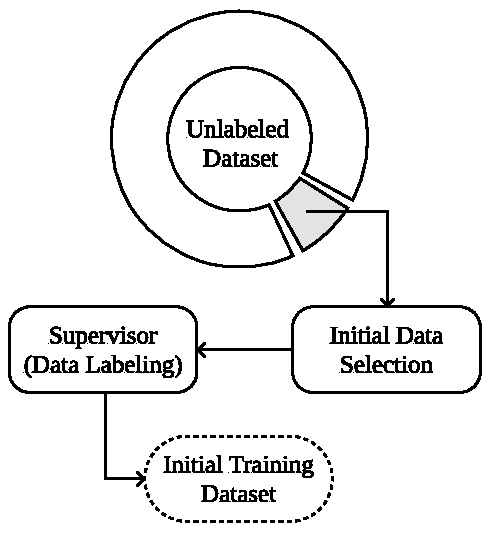
\includegraphics[width=.4\linewidth]{../analysis/al_initialization}
    \caption{%
        Active Learning initialization.
    }~\label{fig:al_initialization}
\end{figure}

Once an initial training dataset is set up, the iterative process of AL takes
place. An AL iteration is completed once a new batch of labeled data is added
to the training dataset. A standard AL process is shown in
Figure~\ref{fig:al_iteration} and is composed of the following
steps~\cite{Su2020, Sverchkov2017}:

\begin{enumerate}

    \item Setting up a classification algorithm and uncertainty criterion. The
        classifier is trained using the labeled dataset (\textit{i.e.,} the
        Current Training Dataset), and is used to predict the class membership
        probabilities of the observations found in the unlabeled dataset. The
        class probabilities are passed into an Uncertainty Criterion, which
        will return the classification uncertainty of the classification
        algorithm for each unlabeled observation. The combination of the
        classifier, along with the uncertainty criterion is sometimes referred
        to as the Query/Acquisition function~\cite{Rosario2020}.

    \item Selecting the top N observations. Since it is not possible to
        determine a priori whether the classifier's prediction is correct or
        not, the N observations with highest uncertainty may have been
        unknowingly correctly classified. However, regardless of the
        classification quality, these observations are expected to provide the
        most meaningful information to train the classifier in the next
        iteration.

    \item Labeling the selected N observations and updating the current
        training dataset with the new training observations. The selected
        observations from the unlabeled dataset are presented to the
        supervisor, which is responsible for manually labeling the
        observations. The new (labeled) training observations are added to the
        training dataset and the iteration is completed.

\end{enumerate}

\begin{figure}[H]
	\centering
	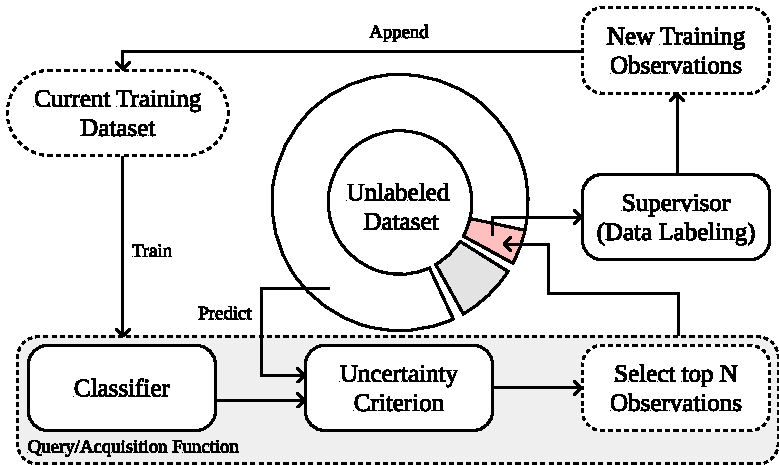
\includegraphics[width=.65\linewidth]{../analysis/al_iteration}
    \caption{%
        Active Learning iteration. In the first iteration, the training set
        collected during the initialization process becomes the ``Current
        Training Dataset''.
    }~\label{fig:al_iteration}
\end{figure}

Two common challenges found in AL implementations is the consistency and
efficiency of AL in practical scenarios~\cite{Kottke2017}. On the one hand,
the consistency problem refers to the high variance in performance (regarding
classification and data selection) over different initializations
(\textit{i.e.,} different initial training datasets) of active learners. On
the other hand, the efficiency problem refers to the maximization of the
quality of the collected data over a run. Therefore, a good active learner is
capable of having a consistent performance over different initializations
while ensuring the production of high-performing classifiers with the least
possible amount of data. There are various factors that may affect the
consistency and efficiency of the AL framework: (1) Human error during data
labeling~\cite{Li2020}, (2) Non-informative initial training
dataset~\cite{Nguyen2004} and (3) Lack of an appropriate uncertainty
criterion~\cite{Rosario2020}. However, AL research typically focuses on either
domain-specific applications of AL, or in the improvement of the AL iterative
process. Query functions can be divided into two different
categories~\cite{Gu2021, Kumar2020}: 

\begin{enumerate}

    \item Informative-based query strategies. These strategies use the
        classifier's output to assess the importance of each observation
        towards the performance of the classifier. These strategies focus on
        quantifying the class uncertainty of the unlabeled observations.
        Since these techniques do not account for the relationships between
        the unlabeled observations and treats each observation
        independently~\cite{Fu2013}.

    \item Representative-based query strategies. These strategies estimate the
        optimal set of observations that will optimize the classifier's
        performance. This strategy contains 3 main approaches: Density-based,
        Diversity-based and Exploration of graph structures. As pointed out
        in~\cite{Kumar2020}, although this method addresses the problem of
        sampling bias and redundant instance selection, these strategies
        typically require more observations in order to reach the desired
        classification performance.

\end{enumerate}

Although there are significant contributions towards the development of more
robust query functions and classifiers in AL, modifications to AL's basic
structure is rarely explored. However, a few studies attempted to do so.
Specifically, in~\cite{Yoo2019} the authors introduce a loss prediction module
in the AL framework to replace the uncertainty criterion. This model
implements a second classifier to predict the expected loss of the unlabeled
observations (using the actual losses collected during the training of the
original classifier) and return the unlabeled observations with the highest
expected loss. Although this contribution is specific to neural networks (and
more specifically, to deep neural networks), they were able to significantly
improve the efficiency of data selection in AL\@. In~\cite{Simeoni2020} the
authors propose the usage of semi-supervised learning during both the
initialization of the AL and the iterative process as well. However, this
method was proposed specifically for deep learning applications.
In~\cite{Fonseca2021}, the authors introduce the generator element in the AL
framework (discussed in Section~\ref{sec:proposed_method}) using an
oversampling method, showing that this method effectively addresses the
limitations of imbalanced learning.  However, this method was implemented
specifically in the Remote Sensing domain and used an oversampling strategy
without consideration for the actual amount of artificial data generated,
which may limit its performance.

\subsection{Query Strategies}

Representative query strategies are less efficient in data selection than
Informative query strategies~\cite{Kumar2020}. However, many studies attempt
to improve its efficiency using 3 main approaches. For
example,~\cite{Huang2014, Li2012, Ienco2013} used a density-based approach
using clustering algorithms to select the observations closest to the centroid
of each cluster. The diversity-based approach was developed to avoid the
selection of redundant observations in batch-mode learning~\cite{Brinker2003}.
Other representative strategies were also developed for graph-based
structures~\cite{Jia2019} which attempt to find the most representative nodes
and edges of a graph network. However, recent research often use
representative approaches alongside informative approaches~\cite{Gu2021,
Samat2016}. 

Informative query strategies, unlike representative query strategies, do not
account for the structure of the unlabeled dataset. As a result, this type of
strategy may lead to the inefficient selection of observations (\textit{i.e.,}
redundant observations with similar profiles)~\cite{Kumar2020}. Research on
more robust selection criteria attempts to address the efficiency problem.
This is motivated by the importance of the selection criteria in AL's
iterative process~\cite{Rosario2020}. Specifically, Settles~\cite{Settles2011}
observed that in some datasets informative query strategies fail to outperform
the random selection of observations. Generally, the Random Selection query
method method is used as a baseline method. This method disregards the class
membership probabilities produced by the classifier and returns N random
points from the dataset without following any specific criteria.

A frequently used query strategy is Uncertainty Sampling, originally proposed
in~\cite{Lewis1994}. Using this method, the estimation of an observation's
uncertainty is based on the target class with the highest probability ($p_a$,
according to the classifier) and the uncertainty is calculated as $1-p_a$.
However, since this method dismissed the classifier's predictions on the
remaining labels, the Breaking Ties criterion was proposed to address this
limitation for multiclass problems~\cite{Luo2005}. This method uses the two
target classes with highest probability ($p_a$ and $p_b$, according to the
classifier) and the uncertainty is calculated as $p_a - p_b$ (in this case,
the lower the output value, the higher the uncertainty). Recent variants of
the Breaking Ties criterion, such as the Modified Breaking Ties, attempted to
fix some limitations of the original method~\cite{Liu2018, Li2012a}.

Another common informative query strategy is the calculation of Shannon's
Entropy. This metric measures the level of uncertainty
based on the probabilities of a set of possible events. Its formula is given
by $H(p)=-\sum_{i=0}^n{p_i\log_2{p_i}}$, having $p$ as the set of
probabilities of all target classes. The application of the Entropy
uncertainty criterion is also frequently applied in Deep Active
Learning~\cite{Aghdam2019}. Other Entropy-based methods were also developed
for more specific applications. For example, an ensemble querying approach
known as Entropy Querying-by-Bagging uses the predictions of all estimators to
find the maximum entropy of each observation~\cite{Abe1998}.

The Query by Committee (QBC) strategy was developed to address ensemble
classifiers. It is a disagreement based strategy attempts to maximize the
information gain at each iteration by computing the disagreement of the
predictions over the estimators that form the ensemble. The Entropy
Querying-by-Bagging (described previously) and Query-by-Boosting methods are
also ensemble strategies. Query by boosting and bagging methods were found to
achieve a good performance over various datasets~\cite{Melville2004}, while
the performance between the two strategies appears to differ significantly
across various scenarios~\cite{Bloodgood2018}.

Other classifier-specific query strategies were also developed for different
applications. However, these methods have the disadvantage of depending on the
classifier being used. For example, Margin Sampling is a well studied strategy
that uses a Support Vector Machine as its classifier in order to select the
unlabeled observations closest to its decision boundaries~\cite{Kumar2020}.
Although, since this method is known to lead to the excessive selection of
observations in dense regions~\cite{Zhou2014}, it was improved in various
ways. In~\cite{Zhou2014} the authors extend this strategy by applying the
manifold-preserving graph reduction algorithm beyond the normal Margin
Sampling method.

\section{Data Augmentation Methods}~\label{sec:data_augmentation}

Data Augmentation methods expand the training dataset by introducing new and
informative observations~\cite{Behpour2019}. The production of artificial data
may be done via the introduction of perturbations on the
input~\cite{Zhong2020}, feature~\cite{DeVries2017} or output
space~\cite{Behpour2019}. Data Augmentation methods may be divided into
Heuristic and Neural Network-based approaches~\cite{Shorten2019}. In addition,
they may also be distinguished based on its generation strategy, whether local
(considers a local/specific subset of the dataset) or global (considers the
overall distribution of the training dataset).
Figure~\ref{fig:data_augmentation_taxonomy} shows the general taxonomy of Data
Augmentation methods. Finding the appropriate Data Augmentation method
generally depends on the domain~\cite{DeVries2017}, although some studies
discuss which methods are more appropriate according to the
domain~\cite{Shorten2019, Iwana2021, Wong2016}.

\begin{figure}[H]
	\centering
	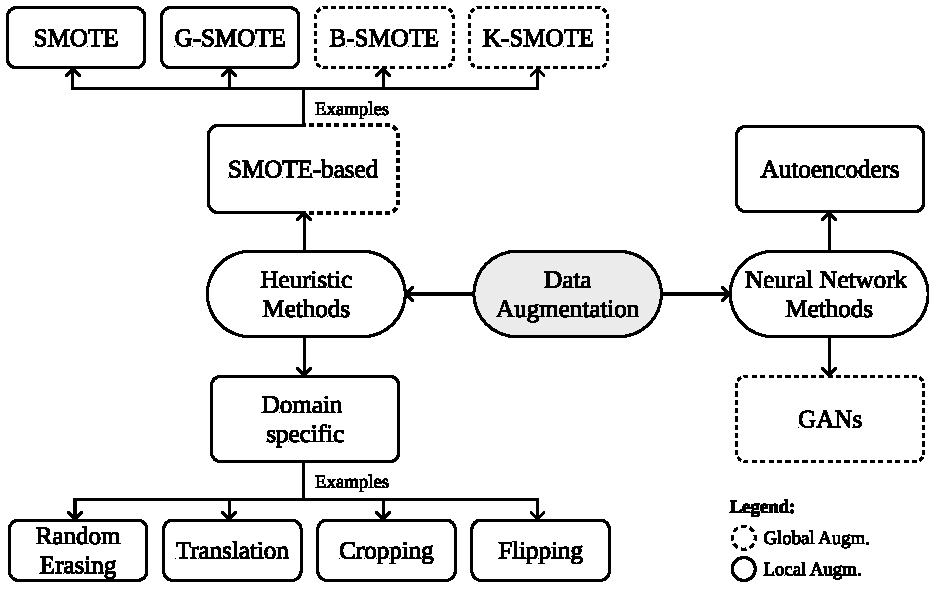
\includegraphics[width=.8\linewidth]{../analysis/data_augmentation_taxonomy}
    \caption{%
        Data Augmentation Taxonomy.
    }~\label{fig:data_augmentation_taxonomy}
\end{figure}

Heuristic approaches attempt to generate new and relevant observations through
the application a predefined procedure, usually incorporating some degree of
randomness~\cite{Kashefi2020}. Since these methods typically occur in the
input space, they require less data and computational power when compared to
Neural Network methods. Neural Network approaches, on the other hand, map the
original input space into a lower-dimensional representation, known as the
feature space~\cite{DeVries2017}. The generation of artificial data occurs in
the feature space and is reconstructed into the input space. Although these
methods allow the generation of less noisy data in high-dimensional contexts
and more plausible artificial data, they are significantly more
computationally intensive. Considering the scope of this paper (the paper's
contribution is described in Sections~\ref{sec:introduction}
and~\ref{sec:proposed_method}), the computational power available for this
experiment and the breadth of datasets used in our experimental procedure, we
will focus on domain-agnostic heuristic data augmentation methods.

While some techniques may depend on the domain, others are domain-agnostic.
For example, Random Erasing~\cite{Zhong2020}, Translation, Cropping and
Flipping are image data-specific augmentation methods. Other methods, such as
most of the variants of the Synthetic Minority Oversampling TEchnique
(SMOTE)~\cite{Chawla2002}, may be considered domain agnostic. However, SMOTE
methods were originally developed as oversamplers, whose goal is to balance
the class frequencies of the target variable in the training dataset and
address the class imbalance bias~\cite{Fonseca2021ksmote}. Therefore,
oversampling methods may be considered a subset of Data Augmentation. Data
Augmentation strategies may follow varying augmentation strategies, which does
not necessarily depend on the target class distribution. An example of the
differences among general data augmentation and oversampling generation
strategies is shown in Figure~\ref{fig:augmentation_strategies}.

\begin{figure}[H]
	\centering
	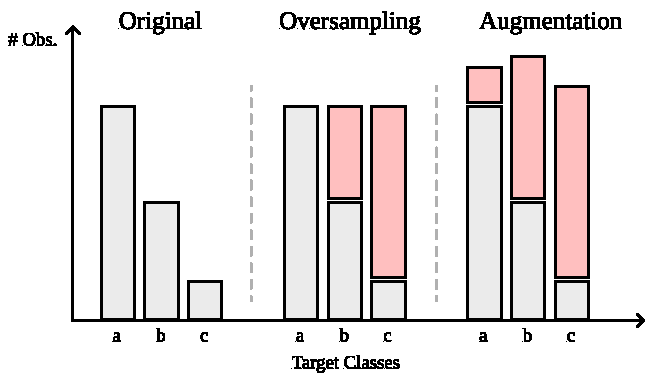
\includegraphics[width=.6\linewidth]{../analysis/augmentation_strategies}
    \caption{%
        Examples of data augmentation Strategies. The salmon-colored bars
        represent artificial data using the normal oversampling (center group) and
        an example of augmentation (right group) strategies.
    }~\label{fig:augmentation_strategies}
\end{figure}

The simplest approach found in the literature is randomly duplicating existing
training observations. As a non-informed data generation method, although
simple to implement, it increases the risk of overfitting and generally
performs worse than other informed heuristic
methods~\cite{Douzas2019imbalanced}.

The SMOTE method generates artificial data via the linear interpolation
between a random observation and one of its $k$-nearest neighbors (also
randomly selected)~\cite{Chawla2002}. Although simple and effective, it also
contains several limitations which motivated the development other variants,
discussed below. Specifically, its selection mechanism does not consider the
global structure of the dataset while its generation mechanism introduces
little variability into the training dataset~\cite{Douzas2019}.
Borderline-SMOTE (B-SMOTE)~\cite{Han2005} improves the selection mechanism by
attributing a larger importance to the observations closer to the decision
boundaries. The selected observations are used to run the SMOTE method in
order to produce better defined decision boundaries. A more recent improvement
of the selection mechanism is K-means SMOTE (K-SMOTE)~\cite{Douzas2018}. This
method uses a clustering-based approach to overcome imbalances between and
within classes, while considering the densities of each region of the input
space.

\begin{figure}[H]
	\centering
	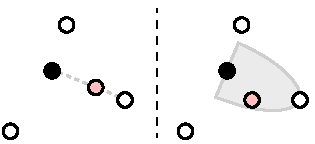
\includegraphics[width=.45\linewidth]{../analysis/smote_vs_gsmote}
    \caption{%
        Examples of data generation using SMOTE and G-SMOTE\@. In this
        example, both G-SMOTE's deformation and truncation parameters assume
        values around $0.5$.
    }~\label{fig:smote_vs_gsmote}
\end{figure}

G-SMOTE~\cite{Douzas2019} modifies SMOTE's generation mechanism. Instead of
generating an observation as a linear combination between 2 others, it
generates observations within an hypersphere defined using the selected
observation as its center and one of its nearest neighbors as its boundary.
The hypersphere contains two hyperparameters, the truncation and deformation
factors, which limit the area of the hypersphere. The difference between SMOTE
and G-SMOTE is shown in Figure~\ref{fig:smote_vs_gsmote}.
Reference~\cite{Douzas2019imbalanced} found that G-SMOTE outperforms various
state-of-the-art oversamplers.

\subsection{Data Augmentation in Active Learning
}~\label{sec:data_augmentation_in_al}

As found in Section~\ref{sec:active_learning_methods}, the improvement of the
AL framework found in the literature are mostly focused on modifications of
the classifier or query strategy. However, a few recent AL applications
implementing data augmentation were found. The method proposed
in~\cite{Kim2021}, Look-Ahead Data Acquisition for Deep Active Learning,
implement image data specific data augmentation to train a deep learning
classifier. However, in this study, data augmentation is based on the
unlabeled observations and occurs before the unlabeled data selection.
In~\cite{Ma2020} the proposed AL method was designed specifically for image
data classification, where a deep learning model was implemented as a
classifier, but its architecture is not described. Other AL frameworks
implementing data augmentation may also be found for Natural Language
Processing applications~\cite{Quteineh2020, Li2021framework}. However, these
methods were designed for specific within that domain and are not necessarily
transferrable to other domains or tasks.

\section{Proposed Method}~\label{sec:proposed_method}

Based on the literature found on AL, most of the contributions and novel
implementations of AL algorithms focused on the improvement of the
choice/architecture of the classifier or the improvement of the uncertainty
criterion. In addition, the resulting classification performance of AL-trained
classifiers is frequently inconsistent and marginally improve the
classification performance when compared to classifiers trained over the full
training set. Finally, in~\cite{Fonseca2021} the authors also found a
significant variability of the data selection efficiency during different runs
of the AL iterative process. In that study the authors proposed a new element
within the AL framework, the generator, which was able to marginally reduce
the variability previously identified. However, this modification was applied
in a Land Use/Land Cover context which contains specific characteristics that
are not necessarily found in other supervised learning problems. Specifically,
high dimensional datasets containing target classes with little data
variability (\textit{i.e.,} cohesive spectral signatures within classes) due
to their geographical proximity. Furthermore, the implementation of the
generator was done using a simple oversampling strategy, which limits the
possibility of employing other techniques with an undefined target amount of
data generated at each iteration.

This paper provides a context-agnostic AL framework towards the integration of
Data Augmentation within AL, with the following contributions:

\begin{enumerate}
    \item Improvement of the AL framework by introducing a parameter
        tuning stage using only the labeled dataset available at the current
        iteration (\textit{i.e.,} no labeled hold-out set is needed).
    \item Generalization of the generator module proposed
        in~\cite{Fonseca2021} from oversampling techniques to any other data
        augmentation mechanism and/or strategy.
    \item Implementation of data augmentation outside of the Deep AL realm,
        which was not previously found in the literature.
    \item Analysis of the impact of Data Augmentation and Oversampling
        in AL over 10 different datasets of different domains, while
        comparing them with the standard AL framework.
\end{enumerate}

The proposed iterative process of the AL framework is depicted in
Figure~\ref{fig:al_proposed}. The generator element becomes an additional
source of data and is expected to introduce additional data variability into
the training dataset. This should allow the classifier to generalize better
and perform more consistently over unseen observations. However, in this
scenario, the amount of data to generate per class at each iteration is
unknown. Consequently, the hyperparameter tuning step was introduced to
estimate the optimal data augmentation strategy at each iteration. In our
implementation, this step uses the current training dataset to perform an
exhaustive search over specified parameters of the generator, tested over a
5-fold cross validation method. The best augmentation strategy found is used
to train the iteration's classifier in the following step.

\begin{figure}[H]
	\centering
	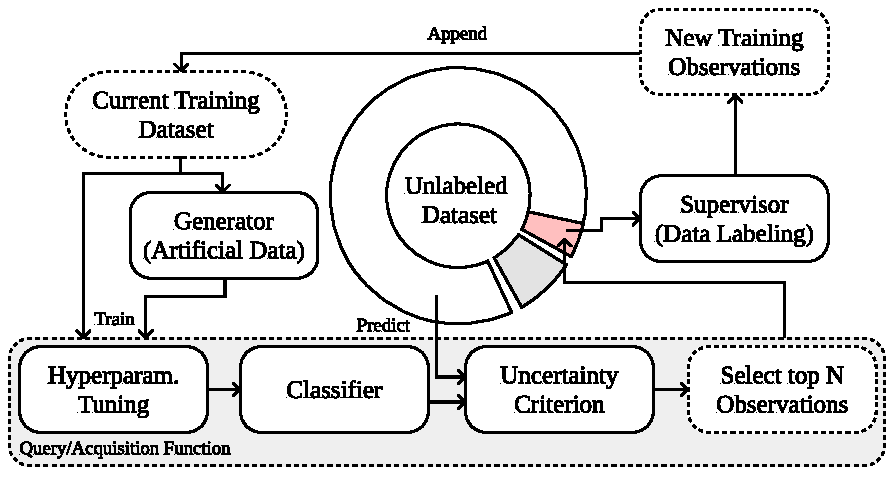
\includegraphics[width=.75\linewidth]{../analysis/al_proposed}
    \caption{%
        Active Learning --- proposed iteration.
    }~\label{fig:al_proposed}
\end{figure}

To show the effectiveness of data augmentation in an AL implementation, we
implemented a simple modification of the G-SMOTE algorithm. This modification
facilitates the usage of G-SMOTE beyond its original oversampling purposes. In
this paper, the data augmentation strategies used ensure the all the class
frequencies are balanced. Furthermore, the amount of artificial data produced
for each class is defined by the \textit{augmentation factor}, which
represents a percentage of the majority class $C_{maj}$ (\textit{e.g.,} an
augmentation factor of $1.2$ will ensure there are $count(C_{maj}) \times 1.2$
observations in every class). In this paper's experiment, the data generation
mechanism is similar to the one in~\cite{Fonseca2021}. This allows the direct
comparison of the two frameworks and establish a causality of the performance
variations to the data generation mechanism (\textit{i.e.,} augmentation vs
normal oversampling) and hyperparameter tuning steps.

This framework was designed to be task-agnostic. Specifically, any data
augmentation method (domain specific or not) may be used, as well as any other
parameter search method. It is also expected to be compatible with other AL
modifications, including the ones that do not affect solely the classifier or
uncertainty criterion, such as the one proposed in~\cite{Yoo2019}.

\section{Methodology}~\label{sec:methodology}

This section describes the different elements included in the experimental
procedure. The datasets used were acquired in open data repositories and its
sources and preprocessing steps are defined in Subsection~\ref{sec:datasets}.
The choice of classifiers used in the experiment are defined in
Subsection~\ref{sec:machine_learning_algorithms}. The metrics chosen to
measure AL performance and overall classification performance are defined in
Subsection~\ref{sec:evaluation_metrics}. The experimental procedure is
described in Subsection~\ref{sec:experimental_procedure}. The implementation
of the experiment and resources used to do so are described in
Subsection~\ref{sec:software_implementation}.

The methodology developed serves 2 purposes: (1) Compare classification
performance once all the AL procedures are completed (\textit{i.e.,} optimal
performance of a classifier trained via iterative data selection) and (2)
Compare the amount of data required to reach specific performance thresholds
(\textit{i.e.,} number of AL iterations required to reach similar
classification performances).

\subsection{Datasets}~\label{sec:datasets}

The datasets used to test the proposed method are publicly available in open
data repositories. Specifically, they were retrieved from
\href{https://www.openml.org/}{OpenML} and the
\href{https://archive.ics.uci.edu/}{UCI Machine Learning Repository}. The
datasets were chosen considering different domains of application, imbalance
ratios, dimensionality and number of target classes, all of them focused on
classification tasks. The goal is to demonstrate the performance of the
different AL frameworks in various scenarios and domains. The data
preprocessing approach was similar across all datasets.
Table~\ref{tab:datasets_description} describes the key properties of the 10
preprocessed datasets where the experimental procedure was applied. 

\begin{table}[H]
    \centering
    \addtolength{\leftskip} {-2cm}
    \addtolength{\rightskip}{-2cm}
    \pgfplotstabletypeset[
        col sep=comma,
        string type,
        every head row/.style={%
            before row=\toprule,
            after row=\midrule
        },
        every last row/.style={after row=\bottomrule},
    ]{../analysis/datasets_description.csv}
    \caption{\label{tab:datasets_description}
        Description of the datasets collected after data preprocessing. The
        sampling strategy is similar across datasets. Legend: (IR) Imbalance
        Ratio
    }
\end{table}

The data preprocessing pipeline is depicted as a flowchart in
Figure~\ref{fig:data_preprocessing}. The missing values are removed from each
dataset by removing the corresponding observations. This ensures that the
input data in the experiment is kept as close to its original form as
possible. The non-metric features (\textit{i.e.,} binary, categorical and
ordinal variables) were removed since the application of G-SMOTE is limited to
continuous and discrete features. The datasets containing over 2000
observations were downsampled in order to maintain the datasets to a
manageable size. The data sampling procedure preserves the relative class
frequency of the dataset, in order to maintain the Imbalance Ratio (IR)
originally found in each dataset (where $IR =
\frac{count(C_{maj})}{count(C_{\min})}$). The remaining features of each
dataset are scaled to the range of $[-1, 1]$ to ensure a common range across
features.

\begin{figure}[H]
	\centering
	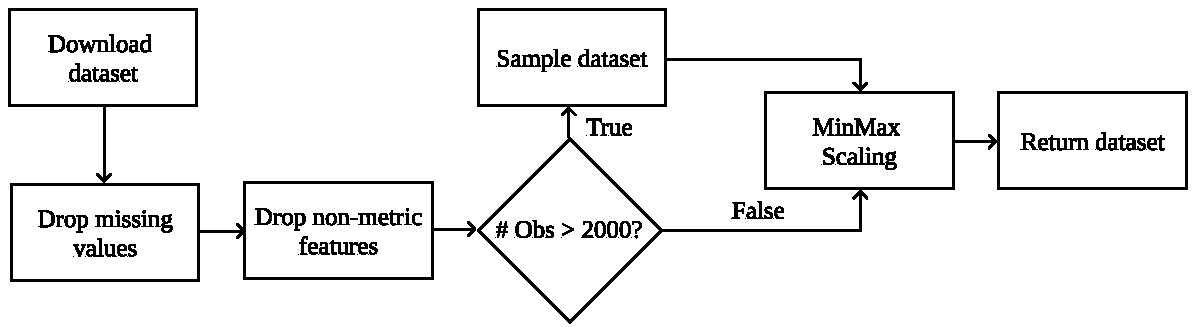
\includegraphics[width=1\linewidth]{../analysis/data_preprocessing}
    \caption{%
        Data preprocessing pipeline.
    }~\label{fig:data_preprocessing}
\end{figure}

The preprocessed datasets were stored into a SQLite database file and is
available along with the experiment's source code in the GitHub repository of
the project (see Subsection~\ref{sec:software_implementation}).

\subsection{Machine Learning Algorithms}~\label{sec:machine_learning_algorithms}

We used a total of 4 classification algorithms and a heuristic data
augmentation mechanism. The choice of classifiers was based on the popularity
and family of the classifiers (tree-based, nearest neighbors-based,
ensemble-based and linear models). Our proposed method was tested using a
Decision Tree (DT)~\cite{Wu1975}, a K-nearest neighbors classifier
(KNN)~\cite{Cover1967}, a Random Forest Classifier (RF)~\cite{Ho1995} and a
Logistic Regression (LR)~\cite{Nelder1972}. Since the target variables are
multi-class, the LR classifier was implemented using the one-versus-all
approach. The predicted class is assigned to the label with the highest
likelihood.

The oversampler G-SMOTE was used as a data augmentation method. The typical
sampling strategy of oversampling methods is to generate artificial
observations on non-majority classes such that the number of majority class
observations matches those of each non-majority class. We modified this
sampling strategy to generate observations for all classes, as a percentage of
the number of observations in the majority class. In addition, the original
G-SMOTE algorithm was modified to accept data selection probabilities based on
classification uncertainty. These modifications are discussed in
Section~\ref{sec:proposed_method}.

Every AL procedure was tested with different selection criteria: Random
Selection, Entropy and Breaking Ties. The baseline used is the standard AL
procedure. As a benchmark, we add the AL procedure using G-SMOTE as a normal
oversampling method, as proposed in~\cite{Fonseca2021}. Our proposed method
was implemented using G-SMOTE as a data augmentation method to generate
artificial observations for all classes, while still balancing the class
distribution, as described in Section~\ref{sec:proposed_method}. 

\subsection{Evaluation Metrics}~\label{sec:evaluation_metrics}

Considering the imbalanced nature of the datasets used in the experiment,
commonly used performance metrics such as Overall Accuracy (OA), although
being intuitive to interpret, are insufficient quantify a model's
classification performance~\cite{Jeni2013}. The Cohen's Kappa performance
metric, similar to OA, is also biased towards high frequency classes since its
definition is closely related to the OA metric, making its behavior consistent
with OA~\cite{Fatourechi2008}. However, these metrics remain popular choices
for the evaluation of classification performance. Other performance metrics
like $Precision = \frac{TP}{TP+TN}$, $Recall = \frac{TP}{TP+FN}$ or
$Specificity = \frac{TN}{TN + FP}$ are calculated as a function of True/False
Positives (TP and FP) and True/False Negatives (TN and FN) and can be used at
a per-class basis instead. In a multiple dataset with varying amount of target
classes and meanings, comparing the performance of different models using
these metrics becomes impractical.

Based on the recommendations found in~\cite{Jeni2013, Kubat1997}, we used 2
metrics found to be less sensitive to the class imbalance bias, along with OA
as a reference for easier interpretability:

\begin{itemize}
    \item The Geometric-mean scorer (G-mean) consists of the geometric mean of
        Specificity and Recall~\cite{Kubat1997}. Both metrics are calculated
        in a multiclass context considering a one-versus-all approach. For
        multiclass problems, the G-mean scorer is calculated as its average
        per class values: 
        
        \begin{equation*}
            \textit{G-mean} = \sqrt{\overline{Sensitivity} \times
            \overline{Specificity}}
        \end{equation*}

    \item The F-score metric consists of the harmonic mean of Precision and
        Recall. The two metrics are also calculated considering a
        one-versus-all approach. The F-score for the multi-class case
        can be calculated using its average per class values~\cite{Jeni2013}:

        \begin{equation*}
            \textit{F-score}=2\times\frac{\overline{Precision} \times
            \overline{Recall}}{\overline{Precision} + \overline{Recall}}
        \end{equation*}

    \item The OA consists of the number of TP divided by the total amount of
        observations. Considering $c$ as the label for the different classes
        present in a target class, OA is given by the following formula:

        \begin{equation*}
            \textit{OA} = \frac{\sum\limits_{c}{\text{TP}_{c}}}{%
		    	      \sum\limits_{c}{(\text{TP}_{c}+\text{FP}_{c})}}
        \end{equation*}
\end{itemize}

The comparison of the performance of AL frameworks is based on its data
selection and augmentation efficacy. Specifically, an efficient data
selection/generation strategy allows the production of classifiers with high
performance on unseen data while using as least non-artificial training data
as possible. To measure the performance of the different AL setups, we follow
the recommendations found in~\cite{Kottke2017}. The performance of an AL setup
will be compared using two AL-specific performance metrics:

\begin{itemize}

    \item Area Under the Learning Curve (AULC). It is the sum of the
        classification performance over a validation/test set of the
        classifiers trained of all AL iterations. To facilitate the
        interpretability of this metric, the resulting AULC scores are fixed
        within the range $[0, 1]$ by dividing the AULC scores by the total
        amount of iterations (\textit{i.e.}, the maximum performance area).

    \item Data Utilization Rate (DUR)~\cite{Reitmaier2013}. Measures the
        percentage of training data required to reach a given performance
        threshold, as a ratio of the percentage of training data required by
        the baseline framework. This metric is also presented as a percentage
        of the total amount of training data, without making it relative to
        the baseline framework. The DUR metric is measured at 45 different
        performance thresholds, ranging between $[0.10, 1.00]$ at a 0.02 step.

\end{itemize}

\subsection{Experimental Procedure}~\label{sec:experimental_procedure}

The evaluation of different active learners in a live setting is generally
expensive, time-consuming and prone to human error. Instead, a common practice
is to compare them in an offline environment using labeled
datasets~\cite{Kagy2019}. In this scenario, since the dataset is already
labeled, the annotation process is done at zero cost.
Figure~\ref{fig:experimental_procedure} depicts the experiment designed for
one dataset over a single run. 

% TODO:
% - Add percentage of observations in each data subset
% - Mention the maximum percentage of data used by the active learners within
%   the train set
A single run starts with the splitting of a preprocessed dataset in 5
different partitions, stratified according to the class frequencies of the
target variable using the K-fold Cross Validation method. During this run, an
active learner or classifier is trained 5 times using a different partition as
the Test set each time. For each training process, a Validation set is created
and is used to measure the data selection efficiency (\textit{i.e.,} AULC and
DUR using the classification performance metrics, specific to AL). The AL
simulations and the classifiers' training occur within the Train set. Once the
training phase is completed, the Test set classification scores are calculated
using the trained classifiers. For the case of AL, the classifier with the
optimal Validation set score is used to estimate the AL's optimal
classification performance over unseen data.

The process shown in Figure~\ref{fig:experimental_procedure} is repeated over
3 runs using different random seeds over the 10 different datasets collected.
The final scores of each AL configuration and classifier correspond to the
average of the 3 runs and 5-fold Cross Validation estimations (\textit{i.e.,}
the mean score of 15 fits, across 10 datasets).

\begin{figure}[H]
	\centering
	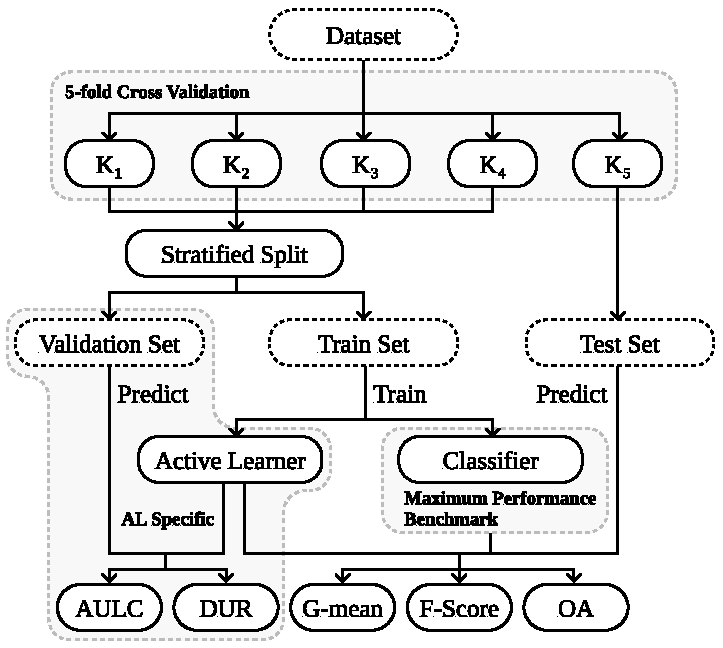
\includegraphics[width=.6\linewidth]{../analysis/experimental_procedure}
    \caption{%
        Experimental procedure flowchart.
    }~\label{fig:experimental_procedure}
\end{figure}

The hyperparameters defined for the AL frameworks, Classifiers and Generators
are shown in Table~\ref{tab:grid}. In the Generators table, we distinguish the
G-SMOTE algorithm working as a normal oversampling method from G-SMOTE-AUGM,
which performs generates additional artificial data on top of the usual
oversampling mechanism. Since the G-SMOTE-AUGM method is intended to be used
with varying parameter values (via within-iteration parameter tuning), the
parameters were defined as a list of various possible values.

\begin{table}[H]
	\centering
	\begin{tabular}{lll}
		\toprule
		Active Learners & Hyperparameters                   & Inputs                         \\
		\midrule
		Standard        & \# initial obs.\                  & 1.6\%                          \\
                        & \# additional obs.\ per iteration & 1.6\%                          \\
                        & max.\ iterations + initialization & 50                             \\
                        & evaluation metrics                & G-mean, F-score, OA            \\
                        & selection Strategy                & Random, Entropy, Breaking Ties \\
                        & within-iteration param.\ tuning   & None                           \\
                        & generator                         & None                           \\
                        & classifier                        & DT, LR, KNN, RF                \\
        Oversampling    & generator                         & G-SMOTE                        \\
        Proposed        & generator                         & G-SMOTE-AUGM                   \\
                        & within-iteration param.\ tuning   & Grid Search K-fold CV          \\
		\toprule
		Classifier      &                                  &                                \\
		\midrule
        DT              & min.\ samples split              & 2                              \\
                        & criterion                        & gini                           \\
		LR              & maximum iterations               & 100                            \\
                        & multi class                      & One-vs-All                     \\
		                & solver                           & liblinear                      \\
                        & penalty                          & L2 (Ridge)                     \\
		KNN             & \# neighbors                     & 5                              \\
                        & weights                          & uniform                        \\
                        & metric                           & euclidean                      \\
		RF              & min.\ samples split              & 2                              \\
		                & \# estimators                    & 100                            \\
                        & criterion                        & gini                           \\
		\toprule
		Generator       &                                  &                                \\
		\midrule
		G-SMOTE         & \# neighbors                     & 4                              \\
                        & deformation factor               & 0.5                            \\
                        & truncation factor                & 0.5                            \\
		G-SMOTE-AUGM    & \# neighbors                     & 3, 4, 5                        \\
                        & deformation factor               & 0.5                            \\
                        & truncation factor                & 0.5                            \\
                        & augmentation factor              & $[1.1, 2.0]$ at 0.1 step       \\
		\bottomrule
	\end{tabular}
    \caption{\label{tab:grid}
        Hyper-parameter definition for the active learners, classifiers and
        generators used in the experiment.
    }
\end{table}

\subsection{Software Implementation}~\label{sec:software_implementation}

The experiment was implemented using the Python programming language, along
with the Python libraries
\href{https://scikit-learn.org/stable/}{Scikit-Learn}~\cite{Pedregosa2011},
\href{https://imbalanced-learn.org/en/stable/}{Imbalanced-Learn}~\cite{JMLR:v18:16-365},
\href{https://geometric-smote.readthedocs.io/en/latest/?badge=latest}{Geometric-SMOTE}~\cite{Douzas2019},
\href{https://research-learn.readthedocs.io/en/latest/?badge=latest}{Research-Learn}
and
\href{https://mlresearch.readthedocs.io/en/latest/?badge=latest}{ML-Research}
libraries. All functions, algorithms, experiments and results are provided in
the \href{https://github.com/joaopfonseca/ml-research/}{GitHub repository of
the project}.

\section{Results \& Discussion}~\label{sec:results_discussion}

In a multiple dataset experiment, the analysis of results should not rely
uniquely on the average performance scores across datasets. The domain of
application and fluctuations of performance scores between datasets make the
analysis of these averaged results less accurate. Instead, it is generally
recommended the use of the mean ranking scores to extend the
analysis~\cite{Demsar2006}. Since mean performance scores are still intuitive
to interpret, we will present and discuss both results. The rank values are
assigned based on the mean scores of 3 different runs of 5-fold Cross
Validation (15 performance estimations per dataset) for each combination of
dataset, AL configuration, classifier and performance metric.

\subsection{Results}~\label{sec:results}

The average ranking of the AULC estimations of AL methods are shown in
Table~\ref{tab:aulc_ranks}. The proposed method almost always improves AL
performance and ensures higher data selection efficiency.

% TODO: 
% - Captions need to be rewritten
% - Convert this table into a bar plot?
\begin{table}[H]
    \centering
    \pgfplotstabletypeset[
        col sep=comma,
        string type,
        every head row/.style={%
            before row=\toprule,
            after row=\midrule
        },
        every last row/.style={after row=\bottomrule},
    ]{../analysis/mean_std_aulc_ranks.csv}
    \caption{%
        Mean rankings of the AULC metric over the different datasets (10),
        folds (5) and runs (3) used in the experiment. The proposed method
        always improves the results of the original framework and on average
        almost always improves the results of the oversampling framework.
    }\label{tab:aulc_ranks}
\end{table}

Table~\ref{tab:aulc_scores} shows the average AULC scores, grouped by
classifier, Evaluation Metric and AL framework. The variation in performance
across active learners is consistent with the mean rankings found in
Table~\ref{tab:aulc_ranks}, while showing significant AULC score differences
between the proposed AL method and the oversampling AL method.

\begin{table}[htb]
    \centering
    \pgfplotstabletypeset[
        col sep=comma,
        string type,
        every head row/.style={%
            before row=\toprule,
            after row=\midrule
        },
        every last row/.style={after row=\bottomrule},
    ]{../analysis/mean_std_aulc_scores.csv}
    \caption{\label{tab:aulc_scores}
        Average AULC of each AL configuration tested. Each AULC score is
        calculated using the performance scores of each iteration in the
        validation set. By the end of the iterative process, each AL
        configuration used a total of XXXX\% instances of the XXXX\% instances
        that compose the training sets.
    }
\end{table}

The average DUR scores were calculated for various G-mean thresholds, varying
between 0.1 and 1.0 at a 0.02 step (45 different thresholds in total).
Table~\ref{tab:optimal_data_utilization} shows the results obtained for these
scores starting from a G-mean score of 0.6 and was filtered to show only the
thresholds ending with 0 or 6. In most cases, the proposed method reduces the
amount of data annotation required to reach each G-mean score threshold.

\begin{table}[H]
    \centering
    \addtolength{\leftskip} {-2cm}
    \addtolength{\rightskip}{-2cm}
    \pgfplotstabletypeset[
        col sep=comma,
        string type,
        every head row/.style={%
            before row=\toprule,
            after row=\midrule
        },
        every last row/.style={after row=\bottomrule},
    ]{../analysis/optimal_data_utilization.csv}
    \caption{\label{tab:optimal_data_utilization}
        Mean data utilization of AL algorithms, as a percentage of the
        training set.
    }
\end{table}

The DUR scores relative to the Standard AL method are shown in
Figure~\ref{fig:dur}. A DUR below 1 means that the Proposed/Oversampling
method requires less data than the Standard AL method to reach the same
performance threshold. For example, running an AL strategy using the KNN
classifier requires 69.6\% of the amount of data required by the Standard AL
method using the same classifier to reach an F-Score of 0.62 (\textit{i.e.,}
requires 30.4\% less data).

\begin{figure}[H]
	\centering
	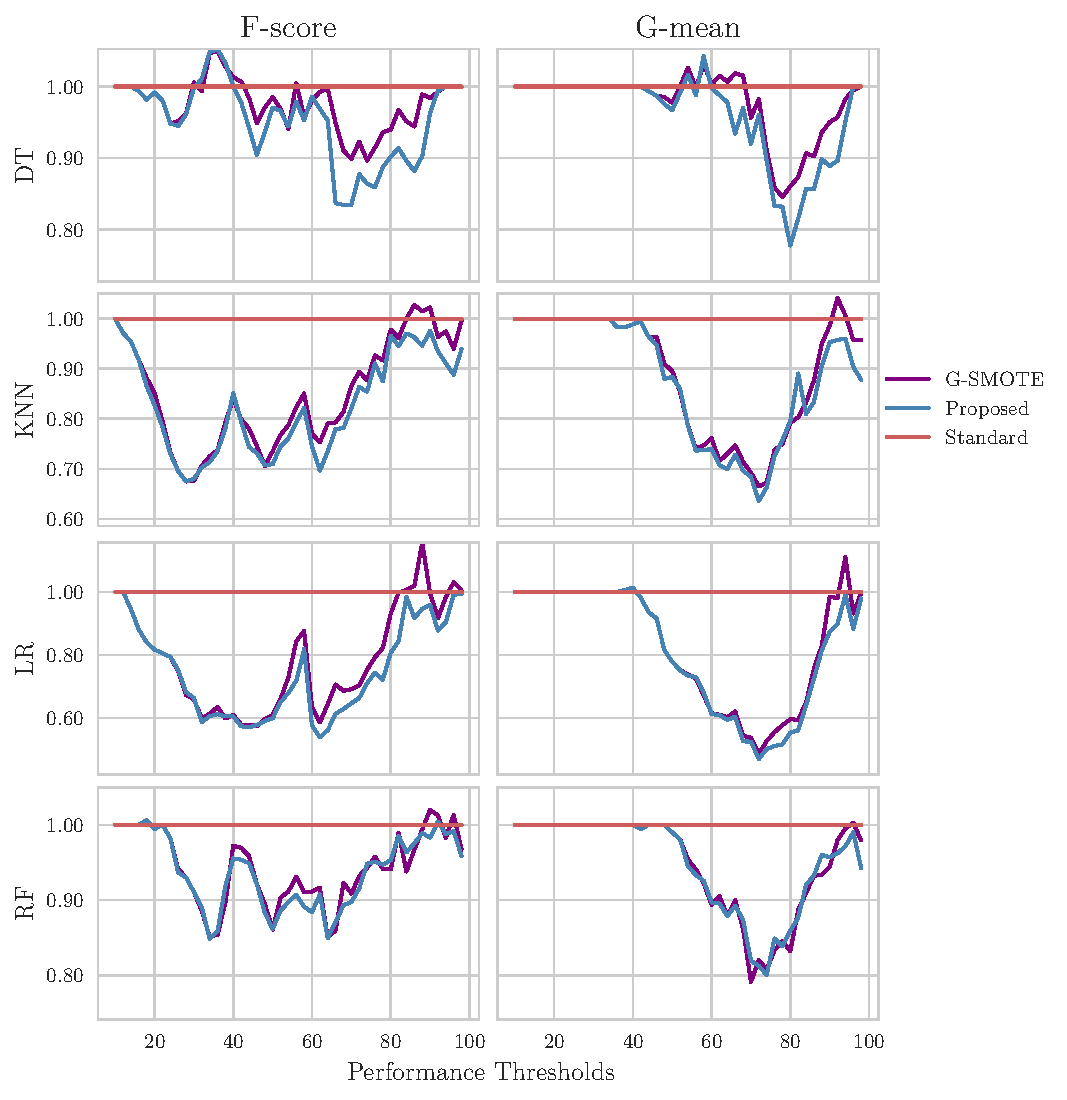
\includegraphics[width=1\linewidth]{../analysis/data_utilization_rate}
    \caption{%
        Mean data utilization rates. The y-axis shows the percentage of data
        (relative to the baseline AL framework) required to reach the
        different performance thresholds.
    }~\label{fig:dur}
\end{figure}

% TODO: Discuss how this technique can be used to train classifiers over fully
% labeled datasets with the sole purpose of increasing their quality.
The mean optimal classification scores of AL methods and Classifiers (fully
labeled training set, without AL) is shown in
Table~\ref{tab:optimal_mean_std_scores}. The proposed AL method produces
classifiers that are almost always able to outperform classifiers using the
full training set (\textit{i.e.,} the ones labeled as MP).

\begin{table}[H]
    \centering
    \addtolength{\leftskip} {-2cm}
    \addtolength{\rightskip}{-2cm}
    \pgfplotstabletypeset[
        col sep=comma,
        string type,
        every head row/.style={%
            before row=\toprule,
            after row=\midrule
        },
        every last row/.style={after row=\bottomrule},
    ]{../analysis/optimal_mean_std_scores.csv}
    \caption{\label{tab:optimal_mean_std_scores}
        Optimal classification scores. The Maximum Performance (MP)
        classification scores are calculated using classifiers trained using
        the entire training set.
    }
\end{table}


% \begin{table}[H]
%     \centering
%     \pgfplotstabletypeset[
%         col sep=comma,
%         string type,
%         every head row/.style={%
%             before row=\toprule,
%             after row=\midrule
%         },
%         every last row/.style={after row=\bottomrule},
%     ]{../analysis/wide_optimal_aulc.csv}
%     \caption{\label{tab:wide_optimal_aulc}
%         AULC scores of each AL configuration tested over the different
%         datasets. Each AULC score is calculated using the G-mean scores of
%         each iteration in the validation set. By the end of the iterative
%         process, each AL configuration used a total of 750 instances of the
%         960 instances that compose the training set.
%     }
% \end{table}


\subsection{Statistical Analysis}~\label{sec:statistical-analysis}

When checking for statistical significance in a multiple dataset context it is
important to account for the multiple comparison problem. Consequently, our
statistical analysis focuses on the recommendations found
in~\cite{Demsar2006}. Overall, we perform 3 statistical tests. The Friedman
test~\cite{Friedman1937} is used to understand whether there is a
statistically significant difference in performance between the 3 AL
frameworks. As post hoc analysis, the Wilcoxon signed-rank
test~\cite{Wilcoxon1945} was used to check for statistical significance
between the performance of the proposed AL method and the oversampling AL
method across datasets. As a second post hoc analysis, the
Holm-Bonferroni~\cite{Holm1979} method was used to check for statistical
significance between the methods using data generators and the Standard AL
framework across classifiers and evaluation metrics.

Table~\ref{tab:friedman_test} contains the \textit{p-values} obtained with the
Friedman test. The difference in performance across AL frameworks is
statistically significant at a level of $\alpha = 0.05$ regardless of the
classifier or evaluation metric being considered.

\begin{table}[H]
	\centering
    \pgfplotstabletypeset[
        col sep=comma,
        string type,
        every head row/.style={%
            before row=\toprule,
            after row=\midrule
        },
        every last row/.style={after row=\bottomrule},
    ]{../analysis/friedman_test.csv}
    \caption{%
        Results for Friedman test. Statistical significance is tested at a
        level of $\alpha = 0.05$. The null hypothesis is that there is no
        difference in the classification outcome across oversamplers.
    }\label{tab:friedman_test}
\end{table}

Table~\ref{tab:wilcoxon_test} contains the \textit{p-values} obtained with the
Wilcoxon signed-rank test. The proposed method was able to outperform both the
standard AL framework, as well as the AL framework using a normal oversampling
strategy proposed in~\cite{Fonseca2021} with statistical significance in 9 out
of 10 datasets.

\begin{table}[H]
	\centering
    \pgfplotstabletypeset[
        col sep=comma,
        string type,
        every head row/.style={%
            before row=\toprule,
            after row=\midrule
        },
        every last row/.style={after row=\bottomrule},
    ]{../analysis/wilcoxon_test.csv}
    \caption{%
        Adjusted p-values using the Wilcoxon signed-rank method. Bold values
        are statistically significant at a level of $\alpha = 0.05$. The null
        hypothesis is that the performance of the proposed framework is
        similar to that of the oversampling or standard framework.
    }\label{tab:wilcoxon_test}
\end{table}

The \textit{p-values} shown in Table~\ref{tab:holms_test} refer to the results
of the Holm-Bonferroni test. The proposed method's superior performance was
statistically significant for any combination of classifier and evaluation
metric. Simultaneously, the proposed method established statistical
significance in the 3 scenarios where the oversampling AL method failed to do
so.

\begin{table}[H]
	\centering
    \pgfplotstabletypeset[
        col sep=comma,
        string type,
        every head row/.style={%
            before row=\toprule,
            after row=\midrule
        },
        every last row/.style={after row=\bottomrule},
    ]{../analysis/holms_test.csv}
    \caption{%
        Adjusted p-values using the Holm-Bonferroni method. Bold values are
        statistically significant at a level of $\alpha = 0.05$. The null
        hypothesis is that the Oversampling or Proposed method does not
        perform better than the control method (Standard AL framework).
    }\label{tab:holms_test}
\end{table}


% TODO: add analysis of dataset complexity versus AL performance


\subsection{Discussion}~\label{sec:sub_discussion}

In this paper we study the application of data augmentation methods through
the modification of the standard AL framework. This is done to further reduce
the amount of labeled data required to produce a reliable classifier, at the
expense of artificial data generation.

% a different data generation strategy
% - Superiority of AL proposed vs standard (AULC + statistical analysis)
In Table~\ref{tab:aulc_ranks} we found that the proposed method was able to
outperform the Standard AL framework in all scenarios. The mean rankings are
consistent with the mean AULC scores found in Table~\ref{tab:aulc_scores},
while showing significant performance differences between the proposed method
and both the standard and oversampling methods. The Friedman test in
Table~\ref{tab:friedman_test} showed that the difference in the performance of
these AL frameworks is statistically significant, regardless of the
classifier or performance metric being used.

% parameter optimization within the iterative process of an AL procedure
% - Discuss consistency of results as compared with other methods (DUR metric)
The proposed method showed more consistent data utilization requirements to
most of the assessed G-mean score thresholds when compared to the remaining AL
methods, as seen in Table~\ref{tab:optimal_data_utilization}. For example, to
reach a G-mean Score of 0.9 using the KNN and LR classifiers, the average
amount of data required with the Oversampling AL approach increased when
compared to the Standard approach. However, the proposed method was able to
decrease the amount of data required in both situations. The robustness of the
Proposed method is clearer in Figure~\ref{fig:dur}. In most cases, this method
was able outperform the Oversampling method. At the same time, the
proposed method also addresses inconsistencies in situations where the
Oversampling method was unable to outperform the standard method.

% Data augmentation vs oversampling
The statistical analyses found in Tables~\ref{tab:wilcoxon_test}
and~\ref{tab:holms_test} showed that the proposed method's superiority was
statistically significant in all datasets except one (Baseball) and
established statistical significance when compared to the Standard AL method
for all combinations of classifier and performance metric, including when the
Oversampling AL method failed to do so. These results show that the Proposed
method increased the reliability of the new AL framework and improved the
quality of the final classifier while using less data.

% Usage of AL as a method to produce better performing classifiers, even in
% settings with fully labeled data
To the best of our knowledge, the method proposed in this paper was the first
AL approach to consistently outperform the maximum performance threshold.
Specifically, in Table~\ref{tab:optimal_mean_std_scores}, the performance of
the classifiers originating from the proposed method was able to outperform
classifiers trained using the full training dataset in all 12 scenarios except
one. This shows that using a meaningful subset of the training dataset along
with data augmentation not only matches the classification performance of ML
algorithms, as it also improves them. Even in a setting with fully labeled
training data, the proposed method may be used as preprocessing method to
further optimize classification performance.

% Future work and limitations
This study introduces data augmentation within the AL framework, along with
the exploration of optimal augmentation methods within AL iterations. However,
the conceptual nature of this study implies some limitations. Specifically,
the large amount of experiments required to test the method's efficacy, along
with the limited computational power available, led to a limited exploration
of the grid search's potential. Future work should focus into understanding
how the usage of a more comprehensive parameter tuning approach improves the
quality of the AL method. In addition, the proposed method was not able to
outperform the standard AL method in 100\% of scenarios. The exploration of
other, more complex, data augmentation techniques might further improve its
performance through the production of more meaningful training observations.
Specifically, in this study we assume that all datasets used follow a
manifold, allowing the usage of G-SMOTE as a data augmentation approach.
However, this method cannot be used into more complex, non-euclidean spaces.
In this scenario, the usage of G-SMOTE is not valid and might lead to the
production of noisy data. Deep Learning-based data augmentation techniques are
able to address this limitation and improve the overall quality of the
artificial data being generated. We also found significant standard errors
throughout our experimental results (see Subsection~\ref{sec:results}), which
is consistent with the findings in~\cite{Fonseca2021, Kottke2017}. This
suggests that the usage of more robust generators did not decrease the
standard error of AL performance. Instead, AL's performance variability is
likely dependent on the quality of its initialization.

\section{Conclusion}~\label{sec:conclusion}

The ability of training ML classifiers is usually limited to the availability
of labeled data. However, manually labeling data is often expensive, which
makes the usage of AL particularly appealing to select the most informative
observations and reduce the amount of required labeled data. On the other
hand, the introduction of data variability in the training dataset can also be
done via data augmentation. However, most, if not all, AL configurations using
some form data augmentation are domain and/or task specific. These methods
typically explore deep learning approaches on both classification and data
augmentation. Consequently, they may not be applicable for other
classification tasks or when the available computational power is
insufficient.

In this paper, we proposed a domain-agnostic AL framework that implements Data
Augmentation and hyperparameter tuning. We found that a simple heuristic Data
Augmentation algorithm is sufficient to significantly improve the data
selection efficiency in AL\@. Specifically, the data augmentation method used
almost always increased AL performance, regardless of the target goal
(\textit{i.e.,} optimizing classification or data selection efficiency). The
usage of data augmentation reduced the amount of iterations required to train
a classifier with a performance as good as (or better than) classifiers
trained with the entire training dataset (\textit{i.e.,} without using AL).
The proposed method was also capable of reducing the size of the training
dataset and use the most informative observations for the training phase of
the classifier, which is expanded with artificial data. 

With this AL configuration, data selection in AL iterations aim towards
observations that optimize the quality of the artificial data produced. The
substitution of less informative labeled data with artificial data is
especially useful in this context, since it allows the reduction of some of
the user interaction necessary to reach a sufficiently informative dataset.
In order to further improve the proposed method future work will (1) focus on
the development of methods with varying data augmentation policies depending
on the different input space regions, (2) develop augmentation-sensitive query
functions capable of avoiding the unnecessary selection of similar
observations from the unlabeled dataset and (3) better understand the gap
between heuristic/input space data augmentation techniques and neural
network/feature space data augmentation techniques in an AL context.

\bibliography{references}
\bibliographystyle{ieeetr}

\end{document}
